\documentclass{article}

% set font encoding for PDFLaTeX or XeLaTeX
\usepackage{graphicx}
\usepackage{ifxetex}
\ifxetex
  \usepackage{fontspec}
\else
  \usepackage[T1]{fontenc}
  \usepackage[utf8]{inputenc}
  \usepackage{lmodern}
\fi
\title{Actividad 5}
\author{Corral Valdez Jesus Giovanni\\
Departamento de Física
}

% Enable SageTeX to run SageMath code right inside this LaTeX file.
% documentation: http://mirrors.ctan.org/macros/latex/contrib/sagetex/sagetexpackage.pdf
% \usepackage{sagetex}

\begin{document}
\maketitle
\section{Traslación de la Tierra}
La traslación es un movimiento en el cual la Tierra viaja alrededor del Sol. La distancia promedio entre estos dos es de 149.60 millones de kilometros, tomando por lo tanto un tiempo total de 365.256 dias en completar su orbita el planeta Tierra.

\section{Calculo de posición}
Es posible calcular la posición de la Tierra alrededor del sol utilizando coordenadas y dando el angulo al cual queremos encontrar su posición. Donde r es la distancia entre la Tierra y el sol (149.60 millones de km)
\begin{equation}
x= r * \cos\theta
\end{equation}
\begin{equation}
y= r * \sin\theta
\end{equation}

\clearpage
\section{Codigo del programa}
\begin{verbatim}
function funcx(g) result (x)
	double precision, intent(in) :: g
	double precision 	     :: x
	 x = 1.496d8 * dcos(g)
end function funcx
function funcy(g) result (y)
	double precision, intent(in) :: g
	double precision 	     :: y
	 y = 1.496d8 * dsin(g)
end function funcy


program traslacion
	implicit none
	integer :: i
	double precision :: g, funcx, funcy
	double precision, parameter :: r = 1.496d8, pi=3.1416d0 !kilometros
	double precision, dimension(1000) :: x, y

 
open (1, file = 'datos.dat', status = 'unknown')
 do i=1, 360, 1
 g = dble(i)
 g = g * pi / 180.0d0
 x(i) = funcx(g)
 y(i) = funcy(g)
 write (1,*) x(i), y(i)
 write (1,*) ' '
 end do
 close (1)


end program traslacion
   
 
\end{verbatim}
\clearpage
\section{Grafica de posición}
\begin{figure}
  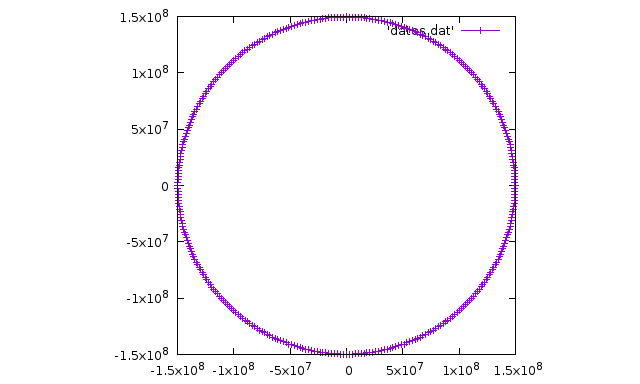
\includegraphics[width=\linewidth]{circulo.png}
  \caption{Grafica de posiciónes.}
\end{figure}


\end{document}
